\documentclass{article}
\usepackage{amsmath}
\usepackage{mathtools}
\usepackage{gensymb}
\usepackage[a4paper,inner=1.5cm,outer=1.5cm,top=2cm,bottom=0.5cm]{geometry} 
\usepackage{xcolor}                    
\usepackage{tikz}                           
\usepackage{multicol}
\usepackage{pgfplots}
\usetikzlibrary{calc}
\usetikzlibrary{intersections}
\usetikzlibrary{intersections,calc,angles,quotes}
\usetikzlibrary{shapes,arrows,positioning,decorations.pathreplacing,calc}
\usetikzlibrary{calc,angles,positioning,intersections,quotes,decorations.markings}
\usepackage{tkz-euclide}
\usetikzlibrary{backgrounds}
\usetikzlibrary{calc,through}
\usetikzlibrary{angles}
\usetikzlibrary{fadings}
\usetikzlibrary{shapes.geometric}
\usetikzlibrary{shapes.symbols}
\usepackage{draftwatermark}
\usepackage{mathptmx}

\SetWatermarkText{\textcolor{black!30}{Mathema Shukur}}
\SetWatermarkFontSize{2 cm}
\usepackage[utf8]{inputenc}
\usepackage{fontspec}

\setmainfont{[Kalpurush.ttf]}
\newfontface{\en}{[Arial.ttf]} %%this is optional, if you want to use a secondary font. Any english font is supported
\newlength\Radius
\setlength\Radius{4cm}
\begin{document} 
	\Large
	\textcolor{red}{Welcome To} 
	\\
	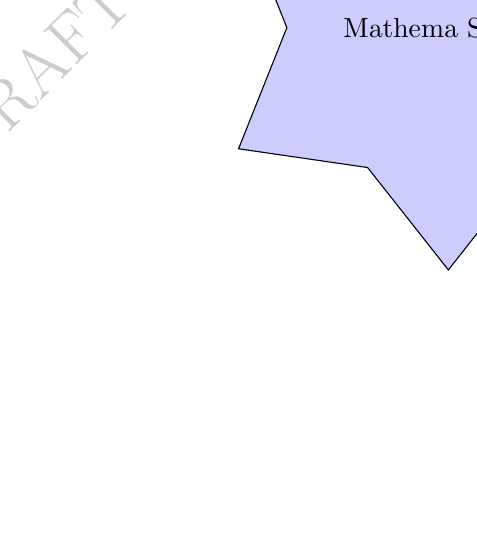
\begin{tikzpicture}
		\tikz \node [fill=blue!20,star,star points=6,draw] {Mathema Shukur };
	\end{tikzpicture}
	\\
	যাদের জন্যে প্রযোজ্যঃ  	\textcolor{magenta}{একাদশ ও দ্বাদশ শ্রেণীর শিক্ষার্থী} \\
	বিষয়ঃ \textcolor{magenta}{উচ্চতর গণিত ১ম পত্র} \\
	অধ্যায়ঃ \textcolor{magenta}{৩-সরলরেখা}\\ 
	Subtopicঃ  \textcolor{magenta}{ বিন্দু হতে রেখার লম্ব দূরত্ব নির্ণয় }\\
	\\
	\textcolor{blue}{$P(x_1,y_1)$ বিন্দু হতে  $ax+by+c=0$ সরলরেখার উপর অঙ্কিত লম্বের দৈর্ঘ্য বা লম্ব দূরত্ব \\ $d=\frac{|ax_1+by_1+c|}{\sqrt{a^2+b^2}}$}\\
	\\
	ঢাকা  বোর্ড-২০২১\\ 
	$(1,1)$ বিন্দু হতে  $4x+3y-22=0$ রেখার  লম্ব দূরত্ব নির্ণয় কর \\
	\\
	$x_1=1,\quad y_1=1,\quad a=4,\quad b=3,\quad c=-22$\\ 
	\\ 
	\begin{align*}
		d&=\frac{|ax_1+by_1+c|}{\sqrt{a^2+b^2}}\\
		\\
		d&=\frac{|(4)(1)+(3)(1)-22|}{\sqrt{(4)^2+(3)^2}}\\
		\\
		d&=\frac{|4+3-22|}{\sqrt{25}}\\
		\\
		d&=\frac{|-15|}{5}\\
		\\
		d&=3
	\end{align*}
	\\
	\begin{tikzpicture}[transform shape,scale=1]
		\draw [-latex,thick](-2,0) -- (7,0) node[right] {$x$} coordinate(x axis);
		\draw [-latex,thick](0,-2) -- (0,10) node[above] {$y$} coordinate(y axis);
		\fill[black] (0,0) circle (1 mm);
		\fill[red] (1,1) circle (1.5 mm);
		\node at (4.5,4) {$\textcolor{green}{4x+3y=22}$};	
		\node at (1,0.5) {$\textcolor{red}{(1,1)}$};	
		\node at (3,2) {$\textcolor{blue}{3}$};	
		\draw[very thick,green] (7,-2)--(-2,10);	
		\draw[very thick,blue,dashed] (1,1)--(3.4,2.8);	
	\end{tikzpicture}
	\\
চট্রগ্রাম, রাজশাহী  বোর্ড-২০২১\\ 
$(\sqrt{3},1)$ বিন্দু হতে  $\sqrt{3}x-y+8=0$ রেখার  লম্ব দূরত্ব নির্ণয় কর \\
\\
$x_1=\sqrt{3},\quad y_1=1,\quad a=\sqrt{3},\quad b=-1,\quad c=8$\\ 
\\ 
\begin{align*}
	d&=\frac{|ax_1+by_1+c|}{\sqrt{a^2+b^2}}\\
	\\
	d&=\frac{|(\sqrt{3})(\sqrt{3})+(-1)(1)+8|}{\sqrt{(\sqrt{3})^2+(-1)^2}}\\
	\\
	d&=\frac{|3-1+8|}{\sqrt{4}}\\
	\\
		d&=\frac{10}{2}\\
		\\
		d&=5
\end{align*}
\\
	\\
\begin{tikzpicture}[transform shape,scale=1]
	\draw [-latex,thick](-7,0) -- (3,0) node[right] {$x$} coordinate(x axis);
	\draw [-latex,thick](0,-4) -- (0,10) node[above] {$y$} coordinate(y axis);
	\fill[black] (0,0) circle (1 mm);
	\fill[red] (1.7,1.019) circle (1.5 mm);
	\node at (-4.5,4) {$\textcolor{green}{\sqrt{3}x-y+8=0}$};	
	\node at (1,0.5) {$\textcolor{red}{(\sqrt{3},1)}$};	
	\node at (-1,2) {$\textcolor{blue}{5}$};	
	\draw[very thick,green] (-6.92,-3.99)--(1.15,9.99);	
	\draw[very thick,blue,dashed] (-2.60,3.5)--(1.7,1.019);	
\end{tikzpicture}
\end{document}